% !TEX encoding = UTF-8 Unicode
\documentclass[a4paper]{report}
\usepackage{tikz}
\usepackage[margin=2.5cm]{geometry}
\usepackage{hyperref}
\usepackage{graphicx}
\usepackage{parskip}
\graphicspath{{figures/}{anotherFigureDirectory/}}
\graphicspath{ {./images/} }
\usepackage{listings}
\usepackage{wrapfig}
\usepackage{float}
\usepackage{color}
\usepackage[school,simplified]{pgf-umlcd}
\definecolor{bluekeywords}{rgb}{0.13,0.13,1}
\definecolor{greencomments}{rgb}{0,0.5,0}
\definecolor{turqusnumbers}{rgb}{0.17,0.57,0.69}
\definecolor{redstrings}{rgb}{0.5,0,0}
\definecolor{gray}{rgb}{0.13,0.13,0.13}
\lstdefinelanguage{FSharp}
                {morekeywords={let, new, match, with, rec, open, module,
                namespace, type, of, member, and, for, in, do, begin, end, fun,
                function, try, mutable, if, then, else},
                keywordstyle=\color{bluekeywords},
                sensitive=false,
                numbers=left,  % where to put the line-numbers;(none, left, right)
                numberstyle=\tiny\color{gray},
                morecomment=[l][\color{greencomments}]{///},
                morecomment=[l][\color{greencomments}]{//},
                morecomment=[s][\color{greencomments}]{{(*}{*)}},
                morestring=[b]",
                showstringspaces=false,
                stringstyle=\color{redstrings}
                }

\title{PoP - Ugeopgave 11}
\author{Christoffer, Inge og Pernille}
\date{\today}

\begin{document}
\maketitle
\tikzstyle{block} = [rectangle, draw, fill=blue!20, text centered,
    rounded corners, minimum height=2.5em]
\tikzstyle{cloud} = [rectangle, draw, fill=white, text centered,
    rounded corners, minimum height = 2em]
\tikzstyle{line} = [draw, -latex]

\subsection*{UML}
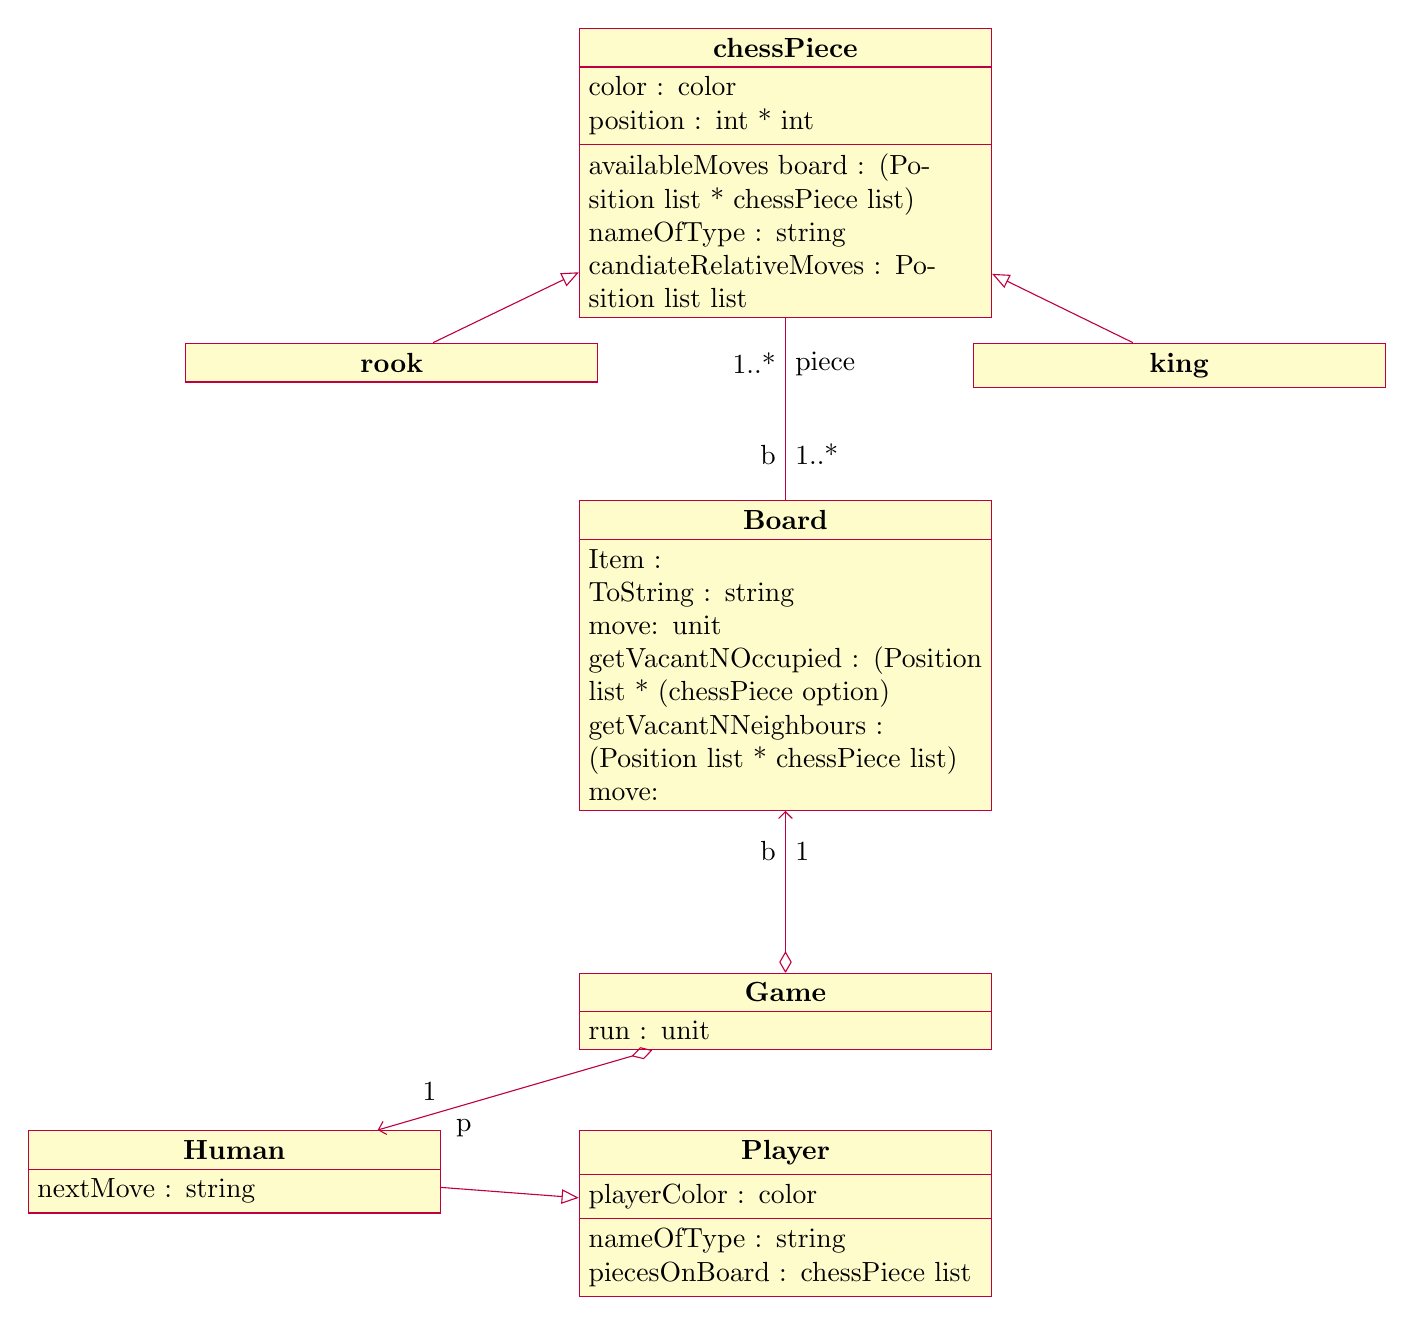
\begin{tikzpicture}
 \begin{class}[text width=5cm]{chessPiece}{0,0}
  \attribute{color : color}
  \attribute{position : int * int}
  \operation{availableMoves board : (Position list * chessPiece list)}
  \operation{nameOfType : string}
  \operation{candiateRelativeMoves : Position list list}
 \end{class}
 \begin{class}[text width=5cm]{rook}{-5,-4}
  \inherit{chessPiece}
 \end{class}
 \begin{class}[text width=5cm]{king}{5,-4}
  \inherit{chessPiece}
 \end{class}
 \begin{class}[text width=5cm]{Board}{0,-6}
  \operation{Item : }
  \operation{ToString : string}
  \operation{move: unit}
  \operation{getVacantNOccupied : (Position list * (chessPiece option)}
  \operation{getVacantNNeighbours : (Position list * chessPiece list)}
  \operation{move: }
 \end{class}
 \association{Board}{b}{1..*}{chessPiece}{1..*}{piece}
 \begin{class}[text width=5cm]{Game}{0,-12}
  \operation{run : unit}
 \end{class}
 \aggregation{Game}{b}{1}{Board}
 \begin{class}[text width=5cm]{Player}{0,-14}
  \attribute{playerColor : color}
  \operation{nameOfType : string}
  \operation{piecesOnBoard : chessPiece list}
 \end{class}
  \begin{class}[text width=5cm]{Human}{-7,-14}
  \inherit{Player}
  \operation{nextMove : string}
 \end{class}
 \aggregation{Game}{p}{1}{Human}
\end{tikzpicture}



\end{document}